\section{Zielsetzung}
In diesem Versuch soll die Funktionsweise eines Sagnac Interferometers kennengelernt werden,
indem zunächst der optische Strahlengang justiert wird. Zudem wird die Abhängigkeit des
Kontrastes vom Polarisationswinkel untersucht, sowie der Brechungsindex von Luft und Glas durch die Messung von
Interferenzeffekten.

\section{Theorie}
\label{sec:Theorie}
\subsection{Beschreibung von Licht}

Licht kann als elektromagnetische Welle beschrieben werden, wobei eine Betrachtung der
elektrischen Feldkomponente aufgrund der Verbindung zwischen elektrischer und
magnetischer Komponente durch die Maxwell Gleichungen ausreicht. \\
Das elektrische Feld ist im Allgemeinen eine vektorielle Größe und kann im Fall von
monochromatischem Licht durch
\begin{equation}
  \vec{E}=\vec{E_0}\exp{\left(i (\omega t-\vec{k}\vec{r})\right)}
\end{equation}
beschrieben werden. Dabei gibt der Vektor $\vec{E_0}$ die Amplitude und Polarisation des Feldes
an. \\
Zwei unterschiedliche Wellen $\vec{E}_1$ und $\vec{E}_2$ lassen sich gemäß des
Superpositionsprinzips addieren, wobei es bei kohärentem Licht, also Licht mit einer festen Phasenbeziehung
zu Interferenzeffekten kommen kann. Diese lassen sich jedoch nicht direkt über die Amplitude
des elektrischen Feldes messen, sondern nur über die Intensität. Diese ist proportional
zu dem zeitlichen Mittelwert des Betragsquadrats des elektrischen Feldes, also
\begin{equation}
  I \propto \langle \lvert \vec{E} \rvert^2 \rangle_t \: .
\end{equation} \\
\subsection{Intensität und Kontrast}

% In diesem Versuch ist die Lichtquelle ein Helium-Neon Laser, dessen Licht eine sehr
% große Kohärenzlänge besitzt, sodass Inteferenzeffekte gut zu beobchten sind.
% Der Lichtstrahl wird bei dieser Art des Inteferometers zunächst über zwei Spiegel auf einen
% verstellbaren Polarisationsfilter gelenkt und anschließend auf einen Polarizing-Beam-Splitter-Cube (PBSC).
% Dieser besteht aus zwei Prismen, die an der Hypothenuse verbunden sind und eine dielektrische Grenzfläche
% aufweisen, sodass ein Teil des Feldes in Abhängigkeit der Polarisation reflektiert wird
% und ein Teil wird transmitiert. Dies führt effektiv zu einer Aufspaltung des Strahls
% in 2 Strahlen, welche sowohl bezüglich der Ausbreitungsrichtun als auch
% bezüglich der Polarisation senkrecht zueinander stehen, wie in Abbildung \ref{fig:PBSC}
% schematisch dargestellt ist. \\
% \begin{figure}{h}
%   \centering
%   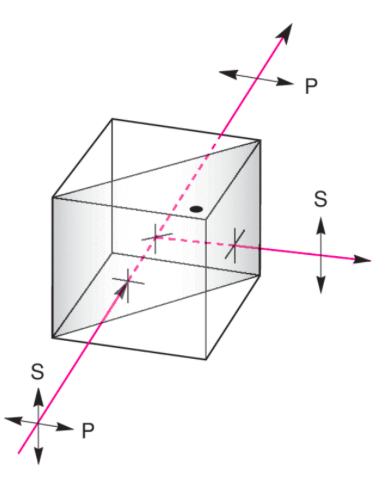
\includegraphics[width=6cm]{PBSC.png}
%   \caption{Schematische Darstellung der Funktionsweise eines PBSC \cite{online1}}
%   \label{fig:PBSC}
% \end{figure}
% Die Strahlen werden über drei weitere Spiegel weitergeleitet und bilden ein Rechteck, welches
% sie in entgegengesetzer Richtung zueinander durchlaufen. Am Ende treffen sie wieder auf den
% PBSC wo sie jedoch keine Interferenzeffekte zeigen, da sie senkrecht zueinander polarisiert sind.
% Nun werden die Strahlen jedoch auf einen weiteren PBSC gelenkt, wo sie nun aufgrund der gemeinsamen
% Polarisationsebene interferieren können. \\




Bei dem Strahlengang des verwendeten Sagnac Interferometers ergibt sich die Intensität der beiden überlagerten Wellen zu
\begin{align}
  I &\propto \langle \lvert
  E_1+E_2 \rvert^2 \rangle_t =
  \langle \lvert E_1 \cos{(\phi)}\cos{(\omega t)} + E_2 \sin{(\phi)}\cos{(\omega t + \delta)} \rvert^2 \rangle_t \\
  &= \frac{1}{2} \bigl( E_{0,1}^2 + E_{0,2}^2 + 2E_{0,1}E_{0,2}\cos(\phi)\sin(\phi)\cos{\delta} \bigr)
\end{align}
mit der Phasendifferenz $\delta$ zwischen den beiden Wellen und dem  Polarisationswinkel $\phi$.
Ob es sich um konstruktive oder destruktive Interferenz handelt, ist abhängig von der Phasendifferenz.
Dabei tritt maximal konstruktive Interferenz auf falls die Phasendifferenz ein ganzes Vielfaches von $2\pi$
ist, also
\begin{align*}
  \delta_{\text{kon}}=2\pi k, \quad k \in \mathbb{Z} \; ,
\end{align*}
wohingegen destruktive Interferenz im Verhältniss dazu um $\pi$ verschoben ist, also
\begin{align*}
  \delta_{\text{dest}}=2\pi(k+1), \quad k \in \mathbb{Z}  \; .
\end{align*}
Somit ergibt sich die maximale bzw. minimale Intensität zu
\begin{equation}
  I_{\text{max/min}} \propto I_{L}(1\pm 2\cos{\phi}\sin{\phi}) \: .
  \label{eqn:imaxmin}
\end{equation}
Falls die beiden Wellen senkrecht zueinander stehen
interferieren sie nicht, da der Interferenzterm $I_{12}$, welcher definiert ist als
$I_{12}= 2 \langle \vec{E_1} \cdot \vec{E_2} \rangle_t$,
verschwindet.\\
Über das Verhältniss der minimalen und maximalen Intensität lässt sich der sogenannte Kontrast
über
\begin{equation}
  V(\phi)= \frac{I_{\text{max}}-I_{\text{min}}}{I_{\text{max}}+I_{\text{min}}}
  \label{eqn:Kontrasttheo}
\end{equation}
definieren, welcher sich nach Gleichung \eqref{eqn:imaxmin} zu
\begin{equation}
  V(\phi)=2\cos{\phi}\sin{\phi}=\sin{2\phi}
\end{equation}
ergibt.
\subsection{Brechungsindex}

Durchläuft einer der beiden Strahlen ein Medium mit einem veränderten Brechungsindex, so
kommt es zu einer Laufzeitdifferenz und somit zu einer veränderten Phasendifferenz,
welche die Interferenz der beiden Strahlen beeinflusst.
Der somit entstandene Phasenversatz $\Delta \Phi$
hängt direkt mit der Anzahl der Interferenzmaxima
\begin{equation}
  M=\frac{\Delta \Phi}{2\pi}
  \label{eqn:AnzMax}
\end{equation}
zusammen, sodass sich über Abzählen der Maxima die entstandene Phasendifferenz bestimmen lässt.
Dies wird in diesem Versuch zur Bestimmung des Brechungsindex zweier unterschiedliche Medien genutzt.
\subsubsection{Brechungsindex von Glas}
Beim Durchlaufen eines Glasplättchens mit Brechungsindex $n$ wird die Phase der Welle durch zwei
unterschiedliche Effekte beeinflusst. Zum einen entsteht eine Phasenänderung aufgrund
des mit dem Brechungsindex verknüpften Laufzeitunterschieds und zudem eine
Phasenverschiebung aufgrund der Brechung des Lichts. Eine einzelne planparallele Platte
mit Brechungsindex $n$ erzeugt für kleine Drehwinkel $\Theta$  näherungsweise eine Phasenverschiebung \cite{skript}
\begin{equation}
\Delta \Phi
(\Theta)=\frac{2\pi}{\lambda_{\text{vac}}}T\Bigl(\frac{n-1}{2n}\Theta^2+\mathcal{O}(\Theta^4)   \Bigr) \; ,
\label{eqn:pM0}
\end{equation}
mit der Dicke $T$ des Plättchens, der Vakuumwellenlänge $\lambda_{\text{vac}}$ des Lasers dem Winkel $\Theta$
zwischen der Plattennormale und dem eintreffenden Strahl.

\subsubsection{Brechungsindex von Gasen}
Falls sich der Brechungsindex $n$ eines Gases von dem der umgebenden Luft unterscheidet, kann es
aufgrund dieser Brechungsindexdifferenz $\Delta n$ ebenfalls zu einer Phasenverschiebung
kommen, wenn nur einer der Strahlen dieses Gas durchläuft.
Dieser Phasenversatz ist dabei anhängig von der Länge $L$
der durchlaufenden Gaszelle und allgemein durch
\begin{equation}
\Delta \Phi(\Theta)=\frac{2\pi}{\lambda_{\text{vac}}} \Delta n\,L
\label{eqn:pM2}
\end{equation}
gegeben \cite{skript}. Der Brechungsindex eines Gases ist dabei über das Lorentz-Lorenz-Gesetz
\begin{equation}
  n \approx \sqrt{1+ \frac{3Ap}{RT}}
  \label{eqn:lorentz}
\end{equation}
mit der Temperatur $T$ und dem Druck $p$ verknüpft, wobei $A$ den molaren Brechungsindex
bezeichnet und $R$ die allgemeine Gaskonstante.
